
\documentclass[12pt]{article}
\setlength{\oddsidemargin}{0in}
\setlength{\evensidemargin}{0in}
\setlength{\textwidth}{6.5in}
\setlength{\parindent}{0in}
\setlength{\parskip}{\baselineskip}
\usepackage{amsmath,amsfonts,amssymb}
\usepackage{graphicx}
\usepackage{enumitem}
\usepackage[]{algorithmicx}
\usepackage{amsthm}
\usepackage{fancyhdr}
\pagestyle{fancy}
\setlength{\headsep}{36pt}
\usepackage{tkz-berge}
\usetikzlibrary{positioning, automata}

\usepackage{hyperref}

\theoremstyle{remark}
\newtheorem*{solution}{Solution}

\newcommand{\makenonemptybox}[2]{%
%\par\nobreak\vspace{\ht\strutbox}\noindent
\item[]
\fbox{% added -2\fboxrule to specified width to avoid overfull hboxes
% and removed the -2\fboxsep from height specification (image not updated)
% because in MWE 2cm is should be height of contents excluding sep and frame
\parbox[c][#1][t]{\dimexpr\linewidth-2\fboxsep-2\fboxrule}{
  \hrule width \hsize height 0pt
  #2
 }%
}%
\par\vspace{\ht\strutbox}
}
\makeatother

\begin{document}
\definecolor {processblue}{cmyk}{0.96,0,0,0}

\lhead{{\bf CSCI 3104, Algorithms \\ Problem Set 6b (40 points)} }
\rhead{Name: \fbox{\phantom{This is a really long name}} \\ ID: \fbox{\phantom{This is a student ID}} \\ {\bf Profs.\ Hoenigman \& Agrawal\\ Fall 2019, CU-Boulder}}
\renewcommand{\headrulewidth}{0.5pt}

\phantom{Test}

\begin{small}
\textbf{Instructions for submitting your solution}:
\vspace{-5mm} 

\begin{itemize}
	\item The solutions \textbf{should be typed} and we cannot accept hand-written solutions. \href{http://ece.uprm.edu/~caceros/latex/introduction.pdf}{Here's a short intro to Latex.}
	\item You should submit your work through \href{https://www.gradescope.com/courses/59294}{\textbf{Gradescope}} only.
	\item If you don't have an account on it, sign up for one using your CU email. You should have gotten an email to sign up. If your name based CU email doesn't work, try the identikey@colorado.edu version. 
	\item Gradescope will only accept \textbf{.pdf} files (except for code files that should be submitted separately on Gradescope if a problem set has them) and \textbf{try to fit your work in the box provided}. 
	\item You cannot submit a pdf which has less pages than what we provided you as Gradescope won't allow it. 
	\item Verbal reasoning is typically insufficient for full credit. Instead, write a logical argument, in the style of a mathematical proof.
	\item For every problem in this class, you must justify your answer:\ show how you arrived at it and why it is correct. If there are assumptions you need to make along the way, state those clearly.
	
	\item You may work with other students. However, \textbf{all solutions must be written independently and in your own words.} Referencing solutions of any sort is strictly prohibited. You must explicitly cite any sources, as well as any collaborators. 
\end{itemize}



\vspace{-4mm} 
\end{small}

\hrulefill

\newpage
\begin{enumerate}




\item (19 pts) Based on the following network and the given edge capacities answer the following. 
\begin{figure}[h!]
\begin{center}
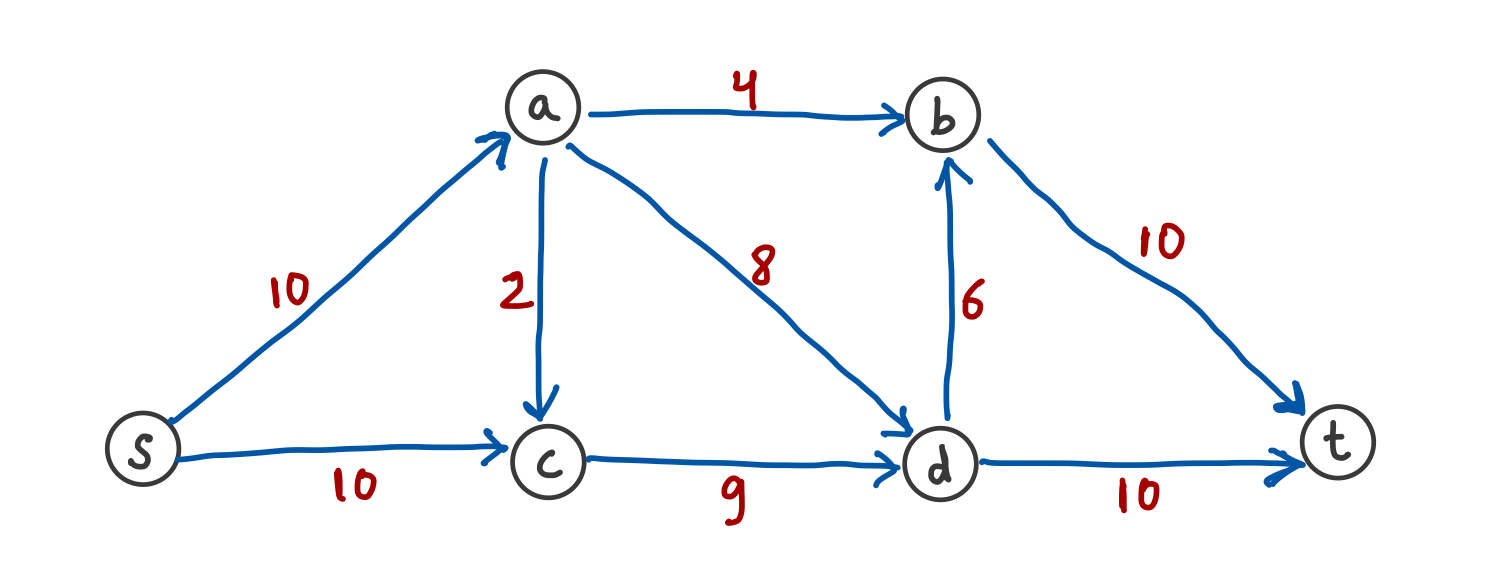
\includegraphics[scale=0.3]{PS6/Flow_6b.jpeg}
\end{center}
\end{figure}

\begin{enumerate}
\item (12 pts) Suppose we start the Ford-Fulkerson algorithm and \textbf{select the path $s->a->c->d->t$ in the first iteration (Do not chose the first s-t path on your own).} Complete all the iterations of Ford-Fulkerson to find the Max-Flow (including the first round that is incomplete).
Clearly show each round with \\
\begin{enumerate}
\item The path that you are selecting in that round.
\item The bottleneck edge on this path.
\item The additional flow that you push from the source by augmenting (pushing maximum allowed flow along) this selected augmenting path.
\item The residual graph with the residual capacities (on both the forward and backward) edges.
\end{enumerate}
Also, report the Max-Flow after the algorithm terminates.

\begin{solution}

\end{solution}

\pagebreak
(more space to solve Q1a)
\pagebreak

\item (3 pts) Show the final flow f(e) for the edges of the original graph when the Ford-Fulkerson algorithm terminates.
\begin{solution}

\end{solution}

\item (4 pts) Find the minimum capacity cut with respect to the capacities on the original graph. Is this minimum capacity equal to the Max-Flow that you earlier identified? Justify your answer in a sentence. Also, report the crossing edges in this cut that are saturated (can't carry any more flow).
\begin{solution}

\end{solution}

\end{enumerate}
\pagebreak

\item (10 pts) Let $(X, Y)$ be any s-t cut in the network $G$ and $a$ be any flow. \begin{enumerate}
    \item (5 pts) Prove that the value of the flow $a$ equals the \textbf{net} flow that crosses the cut $(X, Y)$. \\
    i.e. $value(a)$ = $\sum\limits_{\text{e out of X}}^{}a(e) - \sum\limits_{\text{e in to X}}^{}a(e)$\\	You should use the flow conservation property to complete the proof. \\
    \textbf{Hint :} Recollect the definition of a flow $a$.\\
    $value(a)$ = $\sum\limits_{\text{e out of s}}^{}a(e) - \sum\limits_{\text{e in to s}}^{}a(e)$ where $s$ is the source.
    
    
\begin{solution}

\end{solution}

    \item (5 pts) Use the above proof (from part Q3a) to prove that the value of the flow $a$ $\leq$ Capacity of the cut $(X, Y)$.
\begin{solution}

\end{solution}
\end{enumerate}



\pagebreak

\item (11 pts) CU is organising a spot job fair were many companies participate and take tests to select students. After their final round of interviews, they all find a preference list of candidates that they would like to hire. All the companies just want to hire one student (because recession). All the companies sat together and they realised that if they extend offers to the same students, only one of them would get the student so they decide to run an algorithm to hire the maximum number of students they can together. \\
Example - Following is one such preference of each company after the final round of interviews. If they all give the offer to just their first preference only 3 students will get hired. But a better offer is Apple - Alice, Google - Dave, Facebook - Carol, Amazon - Eliza, Uber - Frank, Netflix - Bob and this gets 6 students hired. \\

Help them come up with an algorithm to find an offer set that gets the maximum students the job using Ford-Fulkerson.
\begin{figure}[h!]
\begin{center}
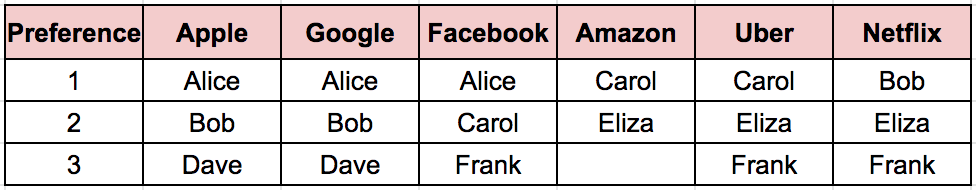
\includegraphics[scale=0.8]{PS6/Job.png}
\end{center}
\end{figure}

\begin{enumerate}
    \item (6 pts) Draw a network $G$ to represent this problem as a flow maximisation problem for the example given above. Clearly indicate the source, the edge directions, the sink and the capacities and label the vertices.
\begin{solution}

\end{solution}

    
    \item (5 pts) Assume that you have access to Fork-Fulkerson sub-routine called \textbf{Ford-Fulkerson(G)} that takes a network and gives out max-flow in terms of f(e) for all the edges. How will you use this sub-routine to find the offer set that employs the maximum number of students. Clearly explain your solution.

\begin{solution}

\end{solution}
\pagebreak
(Space to solve Q3)

\end{enumerate}

\end{enumerate}

\end{document}
